%!TEX root = ../thesis.tex
% ******************************* Thesis Appendix B ********************************

\ifpdf
\graphicspath{{Appendix2/Figs/Raster/}{Appendix2/Figs/PDF/}{Appendix2/Figs/}}
\else
\graphicspath{{Appendix2/Figs/Vector/}{Appendix2/Figs/}}
\fi

\chapter{Supplemental data}
\section{Supplemental figures}

\begin{figure}[H]
  \centering
  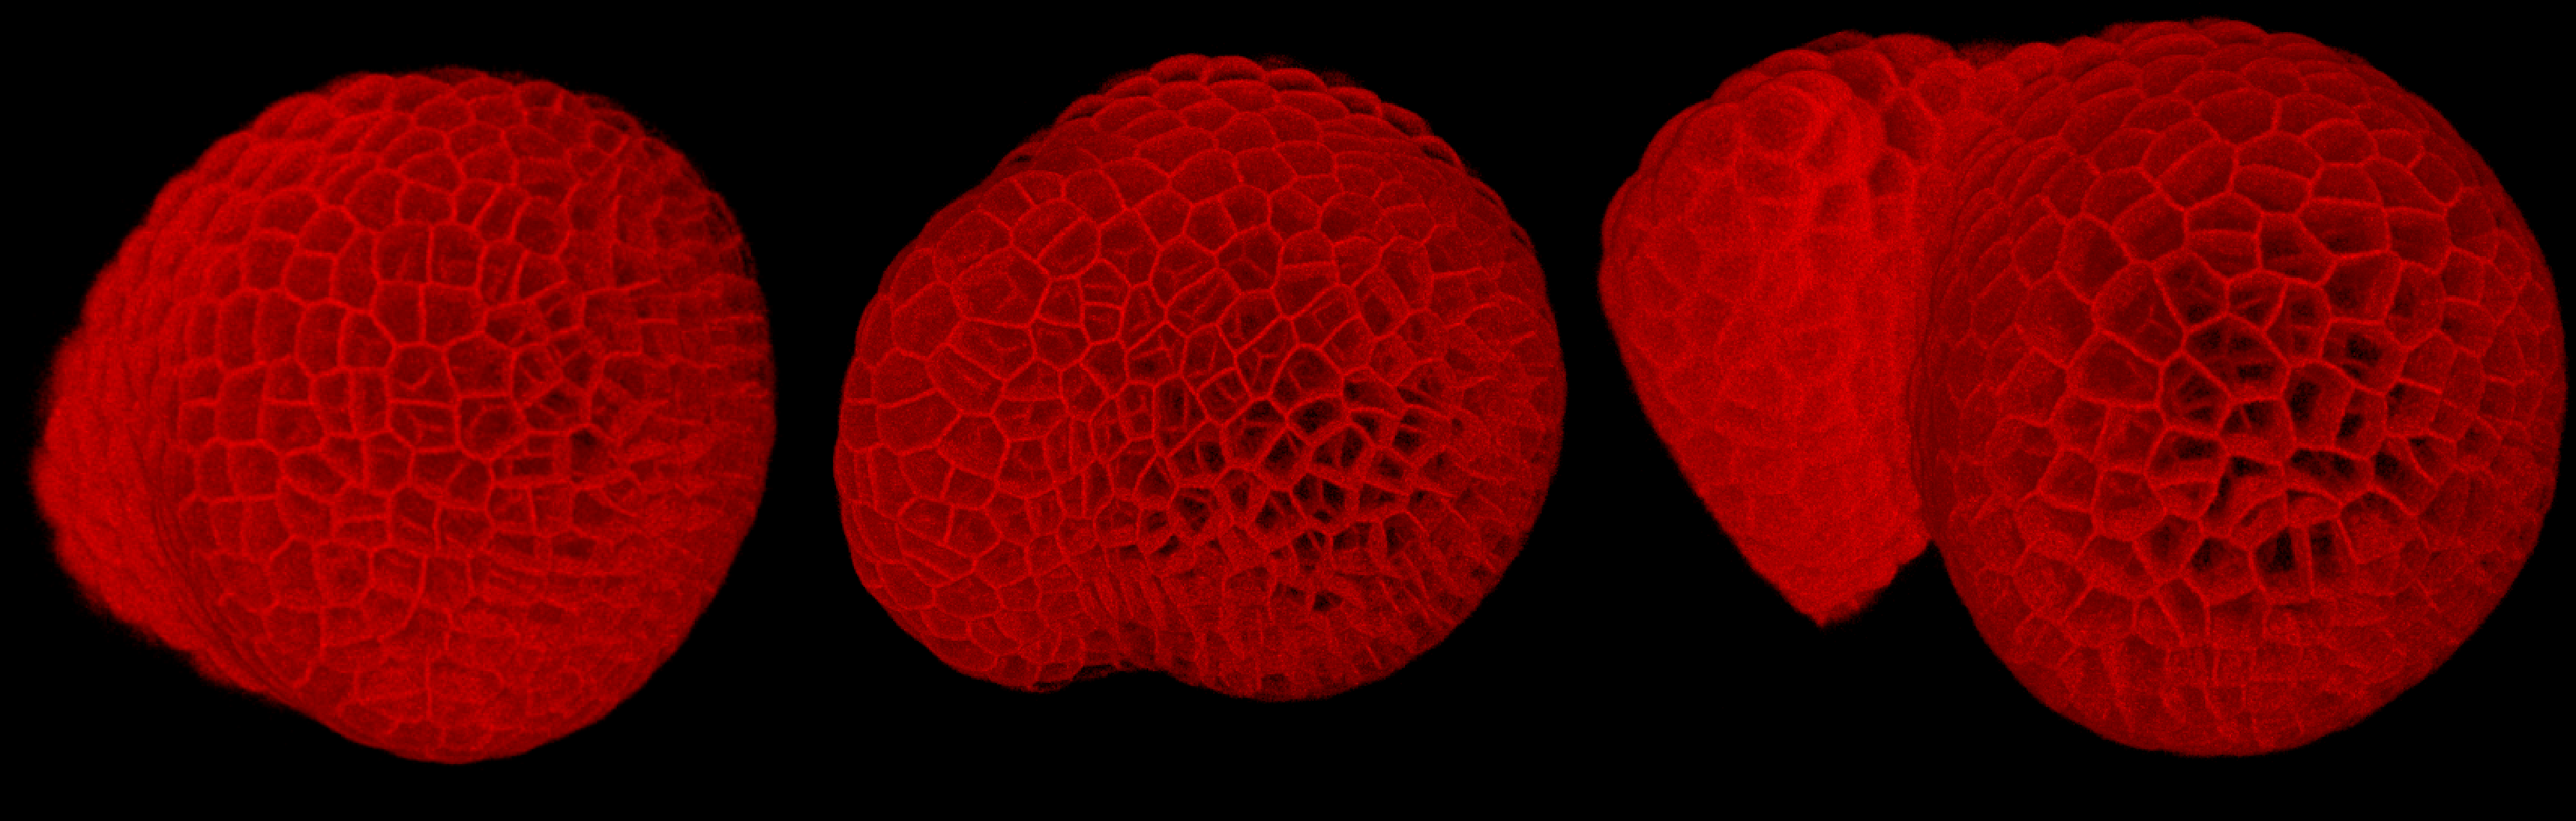
\includegraphics[width=\textwidth]{prim_form.pdf}
  \caption[NPA dilution causes primordia formation]{Membrane channel for plant
    18 at timepoints 0, 36 and 84 hours respectively. In the upper left,
    formation of a primordium throughout the course of the timelapse is clearly
    seen, indicating NPA dilution and reactivation of auxin transport.}
  \label{fig:NPA_primordia}
\end{figure}

\begin{figure}[H]
  \centering
  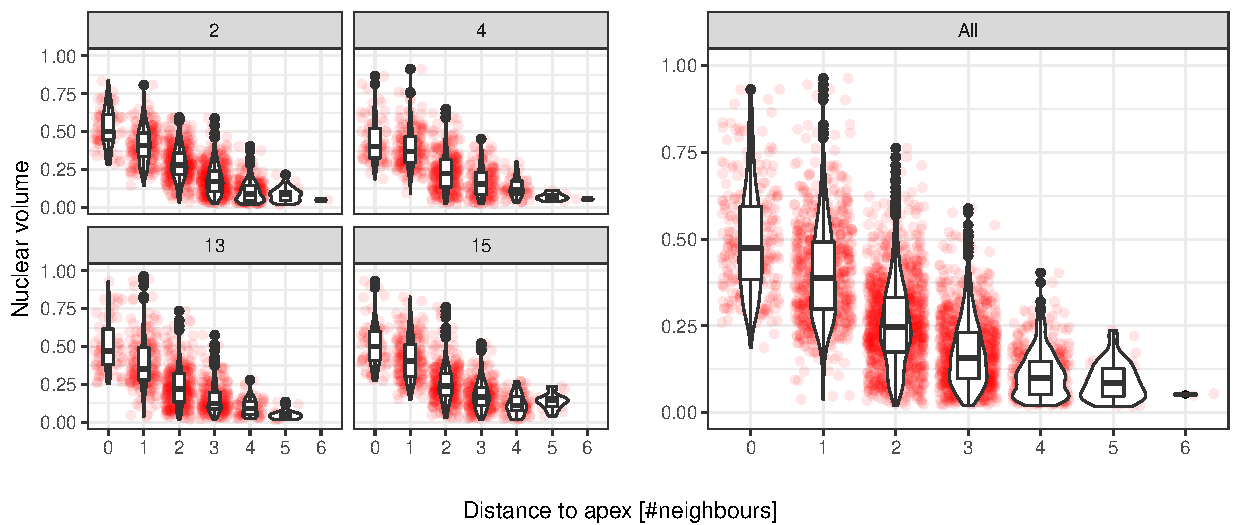
\includegraphics[width=\textwidth]{nvol_apex.pdf}
  \caption[Nuclear volumes at apex]{Distribution of CLV3 nuclear volumes at
    apex, in the epidermis. Lack of data in the periphery is due to CLV3
    loss-of-signal with increasing distance from the CZ. }
  \label{fig:nvol_apex}
\end{figure}

\begin{figure}[H]
  \centering
  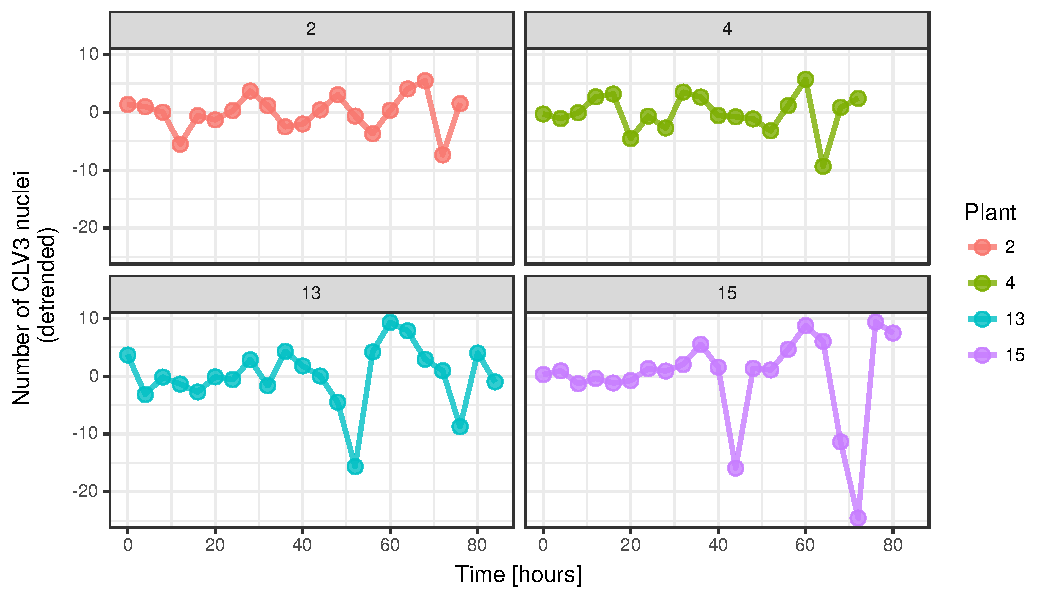
\includegraphics[width=\textwidth]{detrended.pdf}
  \caption[Detrended nuclear trajectories]{Detrended view of trajectories
    visualised in \cref{fig:clv3_trajs}}. The detrending is done by
  subtracting the value curve attained by fitting a second order Loess curve to
  each individual nuclear trace.
  \label{fig:detrended}
\end{figure}

\begin{figure}[H]
  \centering
  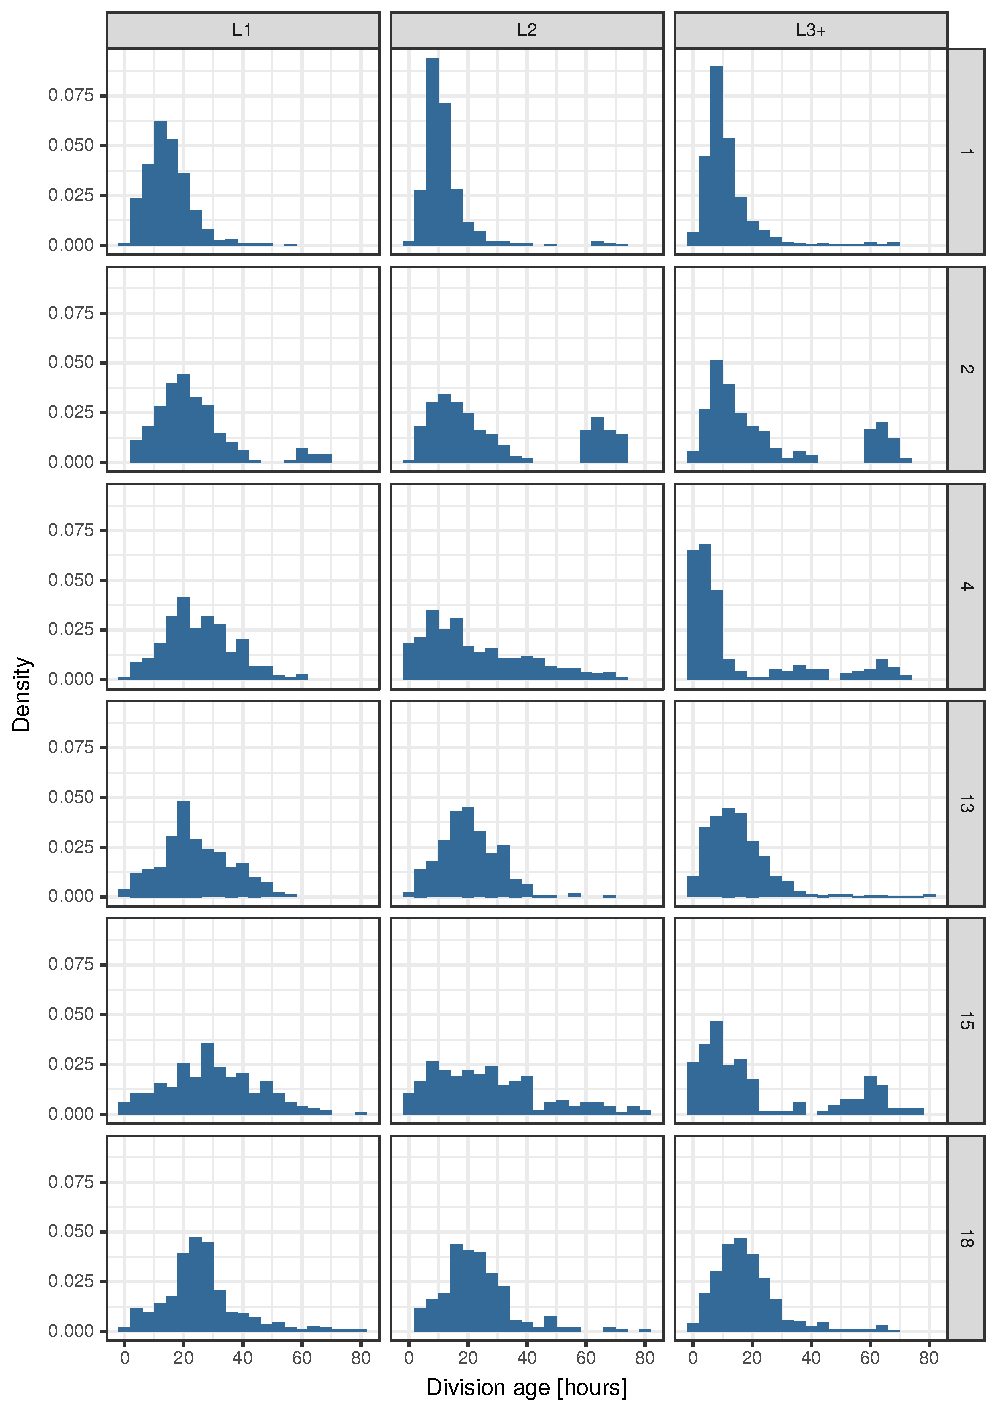
\includegraphics[width=\textwidth]{age_all_plants.pdf}
  \caption[Age distribution, all plants]{Age distribution for all plants,
    showing the general tendency of more cells of higher typically being present
    in the L2 and L3.}
  \label{fig:age_all}
\end{figure}

\begin{figure}[H]
  \centering
  \begin{minipage}[t]{.49\textwidth}
    \centering
    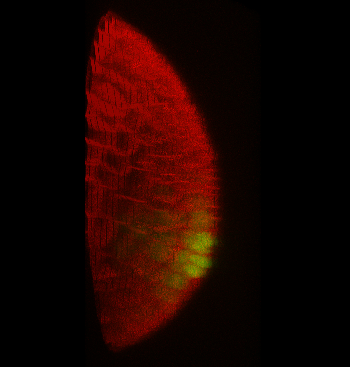
\includegraphics[width=\textwidth]{apexcomp_side.png}
  \end{minipage}
  \begin{minipage}[t]{.49\textwidth}
    \centering
    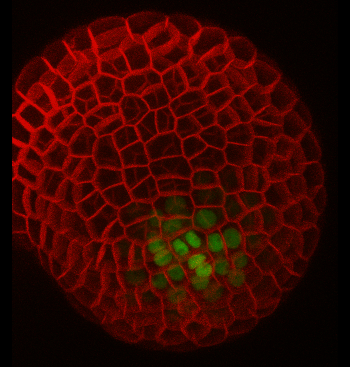
\includegraphics[width=\textwidth]{apexcomp_topview.png}
  \end{minipage}
  \caption[Non-overlapping apices]{Raw data illustration in side view (left) and
    top view (right). The CLV3 peak expression, defining the CLV3 apex, can be
    seen in green, clearly not coinciding with the geometric apex. Example taken
    plant 4, timepoint 48 hours.}
  \label{fig:apex_center}
\end{figure}


\section{Model parameters}
\label{sec:modelparams}
Model parameters for both epidermal models are chosen by visual extraction from
\cref{fig:clv3d2t}. In the simple, WUS activating model of CLV3, we chose our
parameters as
\begin{align*}
  wp &= 5   \\
  wD &= 5   \\
  wd &= 1   \\
  ws &= wD  \\
  Cv &= 150 \\
  Ck &= 2   \\ 
  Cn &= 2   \\
  Cd &= 1   
\end{align*}

where $w$ denotes the WUS protein and $C$ the CLV3 mRNA molecule. Likewise, the
second character denotes the type of reaction. Here, $p$, $D$ and $d$ stand for
the production, diffusion and degradation rate respectively. The $s$ parameter
represents the loss of molecules through the sink, which is set to have the same rate
as the diffusion itself. Other parameters follow those given in the equation
formulation in \cref{sec:modelling_approach}.

For the second model, the parameters are chosen as
\begin{align*}
  wp   &= 5 \\
  wD   &= 2 \\
  wd   &= 1 \\
  ws   &= wD \\
  Cv   &= 150 \\
  Ck   &= 6 \\
  Cn   &= 4 \\
  Cl1k &= 2 \\
  Cl1n &= 4 \\
  Cd   &= 1 \\
\end{align*}
under the same reasoning as above.
